\documentclass[11pt]{article}
% Libraries.
\usepackage{amsmath}
\usepackage{amssymb}
\usepackage{pgfplots}
\usepackage{graphicx}
\usepackage{enumitem}
\usepackage{hyperref}
\usepackage{fancyhdr}
\usepackage{perpage}
\usepackage{float}
\usepackage{esint}
\usepackage{graphicx}
\graphicspath{ {./images/} }

% Property settings.
\MakePerPage{footnote}
\pagestyle{headings}

% Commands
\newcommand{\ti}[1]{\textit{#1}}
\newcommand{\tb}[1]{\textbf{#1}}
\newcommand{\mb}[1]{\mathbb{#1}}
\newcommand{\bx}[0]{\mathbf{x}}
\newcommand{\bv}[0]{\mathbf{v}}
\newcommand{\bw}[0]{\mathbf{w}}
\newcommand{\real}[0]{\mathbb{R}}
\newcommand{\under}[1]{\underline{#1}}
\newcommand{\proof}[0]{\textit{\underline{proof:} }}
\newcommand{\func}[3]{\tb{#1}: {#2} \rightarrow {#3} }
\newcommand{\vx}[0]{\tb{x}}
\newcommand{\vy}[0]{\tb{y}}
\newcommand{\vz}[0]{\tb{z}}
\newcommand{\vo}[0]{\tb{0}}
\newcommand{\va}[0]{\tb{a}}
\newcommand{\vb}[0]{\tb{b}}
\newcommand{\vc}[0]{\tb{c}}
\newcommand{\ve}[0]{\tb{e}}
\newcommand{\vm}[0]{\tb{m}}
\newcommand{\vh}[0]{\tb{h}}
\newcommand{\vf}[0]{\tb{F}}
\newcommand{\vi}[0]{\tb{i}}
\newcommand{\vj}[0]{\tb{j}}
\newcommand{\vk}[0]{\tb{k}}
\newcommand{\vg}[0]{\tb{G}}
\newcommand{\vn}[0]{\tb{n}}
\newcommand{\vu}[0]{\tb{u}}
\newcommand{\vL}[0]{\tb{L}}
\newcommand{\ff}[0]{\tb{f}}
\newcommand{\fg}[0]{\tb{g}}
\newcommand{\rational}[0]{\mathbb{Q}}
\newcommand{\p}[0]{\partial}
\newcommand{\qed}[0]{$\hfill\blacksquare$}
\newcommand{\qerat}{\tag*{$\blacksquare$}}
\newcommand{\lima}{\underset{\vx \rightarrow \va}{\lim}}
\usepackage{amsmath}% http://ctan.org/pkg/amsmath
\newcommand{\notimplies}{%
  \mathrel{{\ooalign{\hidewidth$\not\phantom{=}$\hidewidth\cr$\implies$}}}}


% Attr.
\title{CSC373 \\ Lecture Notes}
\author{Yuchen Wang}
\date{\today}

\begin{document}
    \maketitle
    \tableofcontents
    \newpage
\section{Divide \& Conquer}
\paragraph{General framework}
\begin{enumerate}
	\item Break (a large chunk of) a problem into smaller subproblems of the same type
	\item Solve each subproblem recursively
	\item At the end, quickly combine solutions from the subproblems and/or solve any remaining part of the original problem
\end{enumerate}
\subsection{Master Theorem}
Useful for analyzing divide-and-conquer running time
\paragraph{Theorem}
Let $a \geq 1$ and $b > 1$ be constants, let $f(n)$ be a function, and let $	T(n)$ be defined on the nonnegative integers by the recurrence.
$$T(n) = aT(\frac{n}{b}) + f(n)$$
where we interpret $\frac{n}{b}$ to mean either $\lfloor \frac{n}{b} \rfloor$ or $\lceil \frac{n}{b} \rceil$. Then $T(n)$ has the following asymptotic bounds:
\begin{enumerate}
	\item If $f(n) = \mathcal{O}(n^{\log_b{a-\epsilon}})$ for some constant $\epsilon > 0$, then $T(n) = \Theta(n^{\log_b a})$
	\item If $f(n) = \Theta(n^{\log_b a})$, then $T(n) = \Theta(n^{\log_b a} \lg n)$
	\item If $f(n) = \Omega(n^{\log_b{a+\epsilon}})$ for some constant $\epsilon > 0$, and if $af(\frac{b}{n}) \leq cf(n)$ for some constant $c < 1$ and all sufficiently large $n$, then $T(n) = \Theta(f(n))$.	
\end{enumerate}

\paragraph{Theorem (from CSC236)}
Divide-and-conquer algorithms: partition problem into $b$ roughly equal subproblems, solve, and recombine:
$$T(n) \begin{cases}
	k & \text{if $n \leq B$} \\
a_1T(\lceil n / b \rceil) + a_2T(\lfloor n/b \rfloor) + f(n) & \text{ if $n > B$}
\end{cases}$$
where $b, k >0, a_1, a_2 \geq 0$, and $a = a_1 + a_2 > 0$. \textcolor{red}{$f(n)$ is the cost of splitting and recombining.} If $f$ from the previous slide has $f \in \theta(n^d)$, then
$$T(n) \in \begin{cases}
	\theta(n^d) & \text{if $ a < b^d$} \\
	\theta(n^d\log n) & \text{if $a = b^d$} \\
	\theta(n^{\log_b a}) & \text{if $a > b^d$}
\end{cases}
$$
\subsection{Counting Inversions}
\paragraph{Problem}
Given an array $a$ of length $n$, count the number of pairs $(i,j)$ such that $i < j$ but $a[i] > a[j]$
\paragraph{Applications}
\begin{enumerate}
	\item Voting theory
	\item Collaborative filtering
	\item Measuring the "sortedness" of an array
	\item Sensitivity analysis of Google's ranking function
	\item Rank aggregation for meta-searching on the Web
	\item Nonparametric statistics (e.g., Kendall's tau distance)
\end{enumerate}

\paragraph{Brute Force}
Check all $\theta(n^2)$ pairs

\paragraph{Divide $\&$ conquer}
\begin{enumerate} 
	\item Divide: break away into two equal halves $x$ and $y$
	\item Conquer: count inversions in each half recursively
	\item Combine: \\
	Solve (remaining): count inversions with one entry in $x$ and one in $y$ \\
	Merge: add all three counts
\end{enumerate}

\begin{figure}[h]
	\centering
	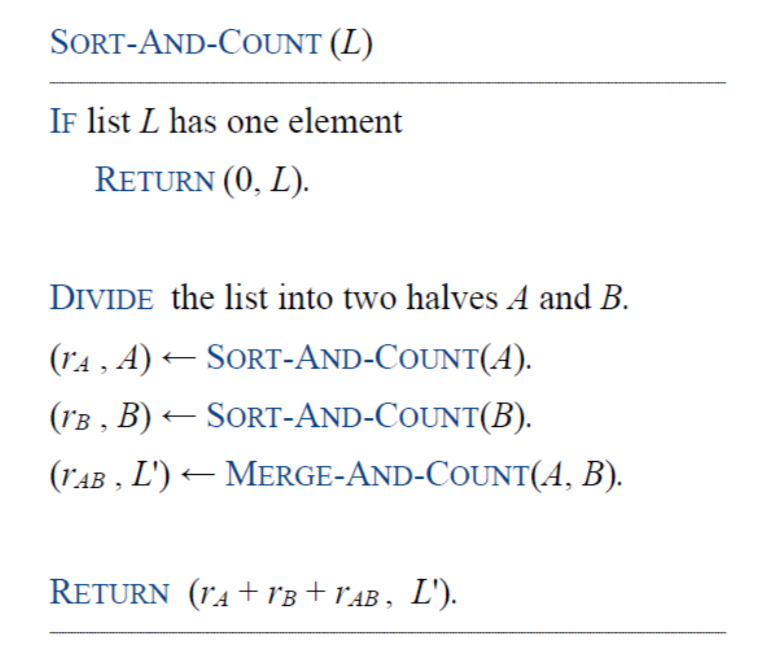
\includegraphics[scale=0.45]{p1}
\end{figure}

Count inversions $(a,b)$ with $a \in A$ and $b \in B$, assuming A and B are sorted:
\begin{enumerate}
	\item Scan A and B from left to right
	\item Compare $a_i$ and $b_j$
	\item If $a_i < b_j$, then $a_i$ is not inverted with any element left in B
	\item If $a_i > b_j$, then $b_j$ is inverted with every element left in A
	\item Append smaller element to sorted list C
\end{enumerate}

\paragraph{How do we formally prove correctness?}
\textcolor{red}{Induction on $n$} is usually very helpful, allows you to assume correctness of subproblems

\paragraph{Running time analysis}
$$T(n) = 2T(\frac{n}{2}) + O(n)$$
Master theorem says this is $T(n) = O(n \log n)$

\subsection{Closest Pair in $\real^2$}
\paragraph{Problem}
Given $n$ points of the form $(x_i, y_i)$ in the plane, find the closest pair of points.
\paragraph{Applications}
\begin{enumerate}
	\item Basic primitive in graphics and computer vision
	\item Geographic information systems, molecular modeling, air traffic control
	\item Special case of nearest neighbor
\end{enumerate}

\paragraph{Brute force running time}
$$\Theta(n^2)$$
\paragraph{Intuition from 1D?}
By sorting and checking, the problem would be easily $\mathcal{O}(n\log n)$
\paragraph{Non-degeneracy Assumption}
No two points have the same $x$ or $y$ coordinate
\paragraph{Closest Pair in $\real^2$}
\begin{enumerate}
	\item Divide: points in equal halves by drawing a vertical line L
	\item Conquer: solve each half recursively
	\item Combine: find closest pair with one point on each side of L
	\item Return the best of 3 solutions
\end{enumerate}

\under{Combine:} We can restrict our attention to points within $\epsilon$ of $L$ on each side, where $\epsilon$ = best of the solutions in two halves

\begin{figure}[h]
	\centering
	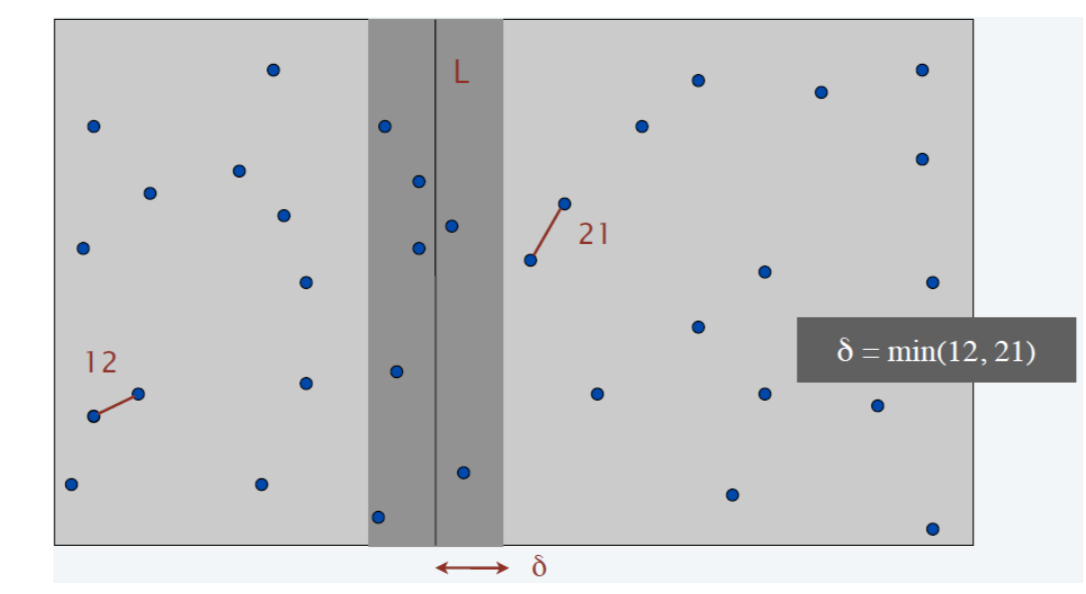
\includegraphics[scale=0.5]{p2}
\end{figure}

\begin{enumerate}
	\item Only need to look at points within $\epsilon$ of $L$ on each side
	\item Sort points on the strip by $y$ coordinate
	\item Only need to check each point with next \textcolor{red}{11} points in sorted list
\end{enumerate}
\paragraph{Why 11?}
Claim: If two points are at least 12 positions apart in the sorted list, their distance is at least $\epsilon$. \\
\proof \\
\begin{enumerate}
	\item No two points lie in the same $\delta / 2 \times \delta / 2$ box
	\item Two points that are more than two rows apart are at distance at least $\delta$
\end{enumerate}

\begin{figure}[h]
	\centering
	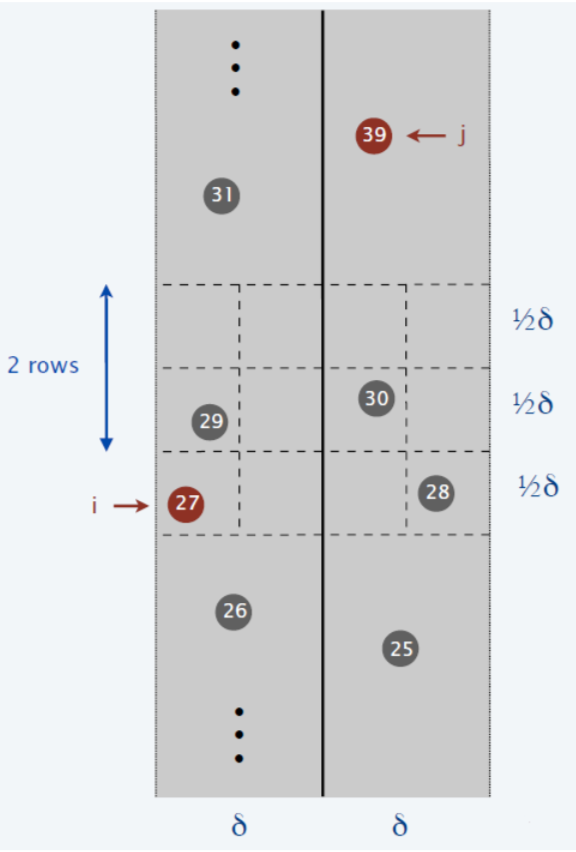
\includegraphics[scale=0.7]{p3}
\end{figure}








\end{document}



